\documentclass[10pt]{article}
\usepackage{enumitem}
\usepackage{hyperref}
\hypersetup{
	colorlinks=true,
	linkcolor=blue,
	filecolor=magenta,      
	urlcolor=cyan,
}
\usepackage{graphicx}
\usepackage{amsmath}
\usepackage[utf8]{inputenc}
\usepackage{mathtools}
\usepackage[caption=false]{subfig}
\usepackage{soul}
\usepackage[top=0.75in, bottom=0.75in, left=0.5in, right=0.5in]{geometry}
\usepackage[margin=1.5cm]{caption}
\usepackage{epsfig,amsmath}
\DeclarePairedDelimiter\abs{${\lvert}$}{${\rvert}$}%
\usepackage{titlesec,color}
\usepackage{kpfonts}
\usepackage{empheq}
\usepackage{palatino}
\usepackage{graphicx,wrapfig}
\setlength{\parskip}{1em}
\setlength{\parindent}{0pt}
\usepackage{array}
\usepackage{gensymb}
\usepackage{soul}
\usepackage{grffile}
\usepackage{multicol}
\usepackage{listings}
\usepackage{color}
\usepackage{tcolorbox}
\usepackage{courier}
\usepackage[T1]{fontenc}
\usepackage{arial}
\usepackage{multicol}
\usepackage[super,sort&compress]{natbib}
\setlength\columnsep{0.3in}
\tcbuselibrary{listings,skins}
\tolerance=1
\emergencystretch=\maxdimen
\hyphenpenalty=10000
\hbadness=1000
\hypersetup{citecolor=black}

\definecolor{dkgreen}{rgb}{0,0.6,0}
\definecolor{gray}{rgb}{0.5,0.5,0.5}
\definecolor{mauve}{rgb}{0.58,0,0.82}

\begin{document}
	
\renewcommand*\rmdefault{phv}
\fontfamily{phv}\selectfont

\newcommand{\avg}[1]{\left<{#1}\right>}
\newcommand{\hence}{\hspace{1cm}\Longrightarrow\hspace{1cm}}
\renewcommand{\ni}{\noindent}
\newcommand{\din}{\indent \indent}
\newcommand{\mni}{\medskip \noindent}
\newcommand{\bni}{\bigskip \noindent}
\newcommand{\sni}{\smallskip \noindent}
\newcommand{\pr}{{\rm Prob}}
\newcommand{\mon}{\begin{displaymath}}
\newcommand{\moff}{\end{displaymath}}
\newcommand{\sumi}[1]{\sum_{{#1}=-\infty}^{\infty}}
\renewcommand{\b}[1]{\mbox{\boldmath ${#1}$}}
\newcommand{\sumy}{\sum_{\b{y}}}
\newcommand{\sumz}{\sum_{\b{z}}}
\newcommand{\pd}[2]{\frac{\partial {#1}}{\partial {#2}}}
\newcommand{\od}[2]{\frac{d {#1}}{d {#2}}}
\newcommand{\odat}[3]{\left. \frac{d {#1}}{d {#2}} \right|_{#3}}
\newcommand{\inti}{\int_{-\infty}^{\infty}}
\newcommand{\eon}{\begin{equation}}
\newcommand{\eoff}{\end{equation}}
\newcommand{\eaon}{\begin{eqnarray}}
\newcommand{\eaoff}{\end{eqnarray}}
\newcommand{\e}[1]{\times 10^{#1}}
\newcommand{\chem}[2]{{}^{#2} \mathrm{#1}}
\renewcommand{\sb}{s}
\newcommand{\s}{s}
\newcommand{\zetaexp}{\left( \zeta e^{q \s t} \right)}
\newcommand{\taunuc}{\tau_{nuc}}
\newcommand{\eq}[1]{Eq. (\ref{#1})}\
\newcommand{\ev}[1]{\langle #1 \rangle}
\newcommand*\mean[1]{${\bar{#1}}$}
\newcolumntype{L}{>{\centering\arraybackslash}m{5cm}}
\bibliographystyle{unsrtnat}


\vspace*{\stretch{1.0}}
\begin{center}
	\LARGE\textbf{MARGO: a Massively Automated Real-time GUI for Object-tracking, a tracking platform for high-throughput ethology}\\
	\large\textbf{}
\end{center}
\vspace*{\stretch{2.0}}
\rightline{\large\textbf{Zach Werkhoven}, \textbf{Gary Qin}, \textbf{Ben de Bivort}}
\rightline{<affiliations>}

\section*{Abstract}

Automated animal tracking offers the potential to probe the biological and environmental effectors of behavior at greater depths than those achievable with comparable manual approaches. Fast tracking in real-time further opens the possibilities of tracking very large numbers of animals or conducting experiments that require closed-loop control for multiple animals in parallel. We developed MARGO, a real-time animal tracking suite for conducting custom behavioral experiments. Here we demonstrate that MARGO can rapidly and accurately track large groups of animals in parallel at a throughput compatible with forward screening. We designed MARGO with simple user interface and flexibility in its tracking implementation. MARGO can be customized to track variety of organisms under diverse imaging conditions with minimal configuration. Additionally, we show that integration of peripheral hardware in MARGO enables closed-loop individual stimulus delivery in high-throughput paradigms. We display MARGO's ability to tightly coordinate tracking and hardware control in parallel with two custom behavioral assays with individually structured trials to quantify phototaxis and optomotor response. In total, MARGO is a flexible platform with the potential to accelerate a wide-variety of behavioral experiments and bring sophisticated stimulus control to the realm of large-scale experimentation.

\vspace{1cm}
\begin{multicols}{2}
\section*{Introduction}

Automated animal tracking methods have become commonplace in behavioral study. Automation affords statistical power and large sample sizes possible, making it invaluable in dissecting out the various determinants of behavior. Though many animal tracking programs exist, few are designed with third-party users in mind and fewer still are generalizable tracking suites that can be flexibly deployed in a variety of experimental contexts. Existing animal trackers vary in computational complexity and specialization to particular imaging configurations. In part, tracker diversity can be attributed to the diversity of behavioral experiment outputs. Trackers can assist in wide range of experimental tasks such as activity monitoring, measuring response to stimuli\cite{Fry_TrackFly_2008,Donelson_High_2012}, and extracting postural information\cite{Mathis_DeepLabCut_2018,Pereira_Fast_2018}. Some trackers are designed to track and maintain identities of multiple individuals occupying the same arena \cite{Prez-Escudero_idTracker_2014,Eyjolfsdottir_Detecting_2014} while others measure the collective activity of populations without maintaining identities \cite{Ramot_The_2008,Swierczek_High_2011,Itskovits_A_2017,Rodriguez_ToxId_2017}. 

Improvements in machine learning approaches to object localization and classification have made it possible to efficiently train models to accurately track and classify a variety of animal species and to visually distinguish identities of individuals across time \cite{Eyjolfsdottir_Detecting_2014,Prez-Escudero_idTracker_2014}. Tracking identity in mixed groups requires resolving identities through collisions where bodies are overlapping. Tracking applications idTracker and FlyTracker train classifiers to assign identities to individuals in each frame and can be used to extract postural information such head and limb position \cite{Eyjolfsdottir_Detecting_2014}. When trained well, these trackers can maintain distinct identities over extended periods with minimal human intervention. Other applications, such as Ctrax and Tracktor\cite{Branson_High_2009,Rodriguez_ToxId_2017,Sridhar_Tracktor_2018}, track animals by segmenting them from the image background and assign identities by stitching traces together across frames but require human intervention to prevent assignment error from propagating over longer timescales. Both approaches offer the ability to study complex social and individual behaviors, but the computational cost of collision resolution means that tracking is generally performed off-line on recorded video data \cite{Liu_A_2018}. Other methods of postural segmentation require manual additional of limb markers or splines fitted in post processing \cite{Kain_Leg_2013,Uhlmann_FlyLimbTracker_2017}. The need separate tracking and recording as well as the spatial resolution required to maintain identities can be rate-limiting for massively high-throughput experiments. Furthermore, the need to record uncompressed or lightly compressed high-resolution video data and the propagation of errors (even at low rates) can make it challenging to track continuously over timescales of days or weeks.

Real-time tracking offers the benefits of closed-loop stimulus delivery and a small data footprint due to the lack of a need to record video data. In general, real-time tracking methods lack the benefit of looking into the future or far into the past offered by off-line tracking on recorded videos \cite{Itskovits_A_2017}. For that reason, real-time multiple animal trackers often rely on spatial segregation of animals to distinguish identities or dispense with identity tracking altogether\cite{Liu_A_2018}. Some existing real-time trackers can track multiple animals in parallel and support a variety of features such as modular arena design, and closed-loop stimulus delivery \cite{Geissmann_Ethoscopes_2017,Straw_Multi_2011,Stowers_Virtual_2017,Chagas_The_2017}. The tracking algorithms, software interface, hardware configurations, and experimental goals of available trackers vary greatly. Some packages such as Tracktor and FlyWorld use a simple application programming interface (API) to implement tracking through background segmentation and match identities across through Hungarian-like Algorithms that minimize frame to frame changes in position. Ethoscopes are an interesting hardware and software solution to high-throughput behavioral experiments and are unique in their support for modular arenas and peripheral hardware for stimulus delivery \cite{Geissmann_Ethoscopes_2017}. Ethoscopes can be networked and operated through a simple web-based interface to conduct real-time tracking based on background segmentation. BioTracker is a flexible tracking platform that offers graphical user-interface (GUI) that allows the user to select different tracking algorithms easily customize tracking parameters \cite{Mnck_BioTracker_2018}. We wanted to develop a platform that could integrate many of these features into a single software package and further build on them to provide a powerful interface for defining custom high-throughput experiments with minimal assumptions about the configuration of the experiment. We wanted to emphasize 1.) fast tracking that could be scalable to very large numbers of individuals or experimental groups over very long time-scales 2.) flexibility to organism, tracking algorithms, experimental paradigms and behavioral arenas 3.) integration of peripheral hardware to enable stimulus driven ethology 4.) accessibility in the user-interface design and data output. 

We developed MARGO, a MATLAB based tracking suite, with these goals in mind. We found that this configuration can reliably track large cohorts of individuals or distinct experimental groups in real-time over very long timescales. Due to its flexible tracking algorithms, it can be used to track individuals when spatially segregated or populations when occupying the same arena. We also demonstrate that tracking requires little to no special hardware and works reliably with minimalist configurations of commonly available equipment. We designed MARGO to require little parameter configuration with good visual feedback on how parameters affect tracking to make it simple and fast to setup new experiments.  Additionally, we demonstrate that integration of peripheral hardware into our tracking suite enables closed-loop individual stimulus delivery in high-throughput paradigms. Using adult fruit flies, we demonstrate two closed-loop applications in MARGO for delivering stimuli to multiple animals in parallel. The first application is an assay for measuring individual phototactic bias in a Y-shaped arena, and the second is an assay for quantifying individual optomotor response. Though MARGO was developed and tested with fruit flies, we show that it can be used to track many small organisms such as fruit fly larvae, nematodes, and larval zebrafish. We believe that MARGO is well-suited to large behavioral screens, experiments requiring real-time stimulus delivery, and users looking to run rapid pilot experiments with little setup. We packaged MARGO with an easy-to-use graphical user interface (GUI) and comprehensive user manual to improve the accessibility of the software and offer it as a resource to the ethology community.

\section*{Results}

\textit{MARGO Description}

In designing MARGO, we decided that it should 1.) facilitate identity preservation by allowing many distinct spatial regions to be tracked independently 2.) tracking accurately and be robust to imaging noise and physical perturbation to enable long-term imaging 3.) have high-throughput with a minimal data footprint to enable large behavioral screens 4.) track high acquisition rate to facilitate tight closed-loop, individual stimulus delivery 5.) work for many organisms, behavioral platforms, and imaging configurations.

The core experimental workflow of MARGO can be briefly summarize as follows: 1.) define spatial regions of interest (ROIs) to track, 2.) construct a background reference image used to separate foreground and background, 3.) sample imaging statistics of clean tracking to facilitate detection and correction of noisy imaging, 4.) perform tracking (Fig. 1A). To address the first design constraint while preserving throughput, we designed MARGO to make it trivial to define hundreds or thousands of spatial regions of interest (ROIs). Tracking ROIs separately offers the ability to preserve identities indefinitely without the need to manually resolve collisions, and can facilitate accurate tracking with very few assumptions about the size and morphology of tracked objects. This fact dramatically improves the throughput of large experiments where accurately maintaining identity is important not only by limiting tracking time to the duration of acquisition but also by removing the requirement for human supervision and intervention. We found that insisting on ROI definition ultimately relaxes the computational requirements enough that thousands of individuals can plausibly be tracked in real-time. This ROI-based architecture can also be used to distinguish population identities rather than individual identities by segregating populations into separate arenas. This configuration therefore allows multiple populations, as well as individuals, to be tested in parallel. To fully take advantage of the throughput offered by tracking thousands of ROIs, we insisted on strategies of ROI definition that would make it simple to rapidly define thousands of ROIs. MARGO initiates tracking setup by defining ROIs through one of two modes. The first is an automated detection mode that detects and segments regular patterns of high-contrast regions in the image. The second mode prompts the user to manually place grids of ROIs of any arbitrary dimensions. In practice, we find that ROI definition typically takes a few seconds but can take as long a few minutes.

Following ROI definition, a background reference image is constructed for each ROI separately. Tracking is performed using a well-known strategy that consists of segmenting binary blobs from a thresholded difference image computed by subtracting the current frame from the background (Fig. 1B). Background subtraction commonly suffers from two issues with opposing solutions. The first is that subtle changes in the background over time introduce noise in the difference image, requiring continuous averaging or reacquisition of the background reference. The second issue is that continuous reacquisition of the background can cause inactive animals to become part of the background rather than foreground. Constructing the reference for each ROI separately mitigates these concerns by allowing the reference to be constructed in a piece-meal fashion when the animals are guaranteed not to become part of the background. Once a background reference is established, tracking can begin. Candidate blobs in the foreground are filtered by size and sorted to ROIs by spatial location. ROIs with multiple candidates are assigned the best candidates based on minimizing frame to frame changes in position.

Degradation of difference image quality over time due changes in the background, noisy imaging, and physical perturbation of the imaging setup constitutes a significant barrier to long term tracking \cite{Sridhar_Tracktor_2018}. The sensitivity of difference images to minor frame to frame changes makes them particularly well suited to low-resolution tracking on complex backgrounds but also exposes the tracking to noise introduce by small changes in the image background. To address this problem, MARGO continuously monitors the quality of the difference image and updates or reacquires the background reference when imaging becomes noisy. Prior to tracking, the software samples the distribution of the total number of above-threshold pixels under clean imaging conditions to serve as a baseline for comparison.  During tracking, the software then continuously calculates statistics on a similar distribution acquired on a rolling basis.  Re-referencing is triggered when the rolling sample significantly deviates from the baseline distribution.

\textit{MARGO is accurate and robust to noise}

We assessed the ability to MARGO to handle degradation of the difference image by repeatedly shifting the background reference by a small amount to simulate misalignment caused by physical perturbation. Tracking was performed live on unaltered image data to serve as a ground truth while simultaneously recording video data. Background misalignment was repeatedly triggered on a fixed interval by shifting the background reference by 2 pixels in a random direction. Trial triggered averaging of the tracking error shows that MARGO reliably detects the misalignment and fully recovers clean tracking typically within 1 second (Fig. 2D). Forcing reacquisition of the background reference has the disadvantage of initializing the reference with a single image, meaning that a median reference image cannot be computed until subsequent references are acquired. We found that this typically causes a reduction in tracking accuracy that is brief (<2s) and had little effect on the overall correlation of the tracking data to the ground truth (r=0.99). Indeed we found a small effect on tracking error (mean 3.07+- 2.5 pixels) even when shifting the background every 2 seconds. In practice, noise-induced background reacquisition is quite rare, occurring less than 10 times over the duration of a two hour experiment.

We tested MARGO's sensitivity to video compression by compressing and tracking a video previously captured during a real-time tracking session. The error of traces from compressed video were calculated by comparing them to the ground-truth traces acquired on uncompressed images in real-time. MARGO showed sub-pixel error in tracking up to 3000-fold compression, a remarkable level stability considering a mean area of 15 pixels for each animal (Fig. 2A). We further tested the robustness of MARGO to noisy imaging by artificially injecting noise into the threshold image of each frame of a video previously acquired and tracked under clean conditions. We injected noise into each frame by randomly setting each pixel to True with a uniform probability. Noise was added to the binary image downstream of noise correction and upstream of tracking to simulate tracking under conditions where noise detection and correction are poorly calibrated. Tracking error was measured as the deviation in tracked positions between each frame of the video with added noise and the unaltered source video.  Even in the absence of noise correction, we measured sub-pixel level error up to 20\% noise (fig. 2B). In practice, we find it easy to create imaging conditions with noise levels well below the levels tested without the use of sophisticated tracking setups.

We fed uncompressed video captured during a live tracking session in MARGO into Ctrax, a popular open-source tracking software package, to measure the error between the two sets of traces. Overall we found a high degree of agreement between traces acquired in MARGO and Ctrax (Fig. 2E-F). Most disagreement we found between the two we attribute to minor variations in blob size and shape arising from differences in background models and segmentation from the background. It is worth noting that although Ctrax flagged many frames for manual inspection and resolution, we opted not to resolve these frames and instead restricted our analysis to automatically acquired traces. Manual inspection of individual frames with error larger than 1 pixel revealed that most major discrepancies occurred in one of two ways 1.) short periods between the death and birth of two traces on the same animal in Ctrax 2.) identity swaps in Ctrax between neighboring animals.

\textit{MARGO is well-suited to massive behavioral screens}

We designed MARGO with high-throughput behavioral screens in mind, where hundreds or thousands of animals may need to be tested from hundreds of experimental groups each. Many features of MARGO have been included to reduce the time needed to establish successful tracking. MARGO includes utilities to visualize object statistics and the effects of adjusting various tracking parameters. Additionally, we added the ability to save and load parameter and experimental configurations into the GUI, facilitating a "one-off" tracking setup and consistency of parameters across experiments. We found that features such visual feedback on parameters, parameter profile loading GUI, automated ROI detection, and the lack of model training in MARGO's tracking algorithm  all substantially reduce the time needed to setup tracking. 

The speed of the tracking algorithm also makes it possible to track very large numbers of animals simultaneously in a single field of view, meaning that multiple experimental groups can be tested simultaneously by a single machine. The mean acquisition rate was measured while systematically varying the number of tracked ROIs to assess MARGO’s capacity for massively high-throughput experiments. We found that the time complexity of the core tracking routine scaled linearly as a function of the number of ROIs tracked [fig. 2]. On modern computer hardware (intel i7 4.0Ghz CPU), we measured acquisition rates above 5Hz up to 2400 ROIs and reached as high 160Hz for single ROI tracking. Achieving an appropriate frame rate will of course depend on the timescale of the targeted movement dynamics. We found that frame rates above 5Hz were more than sufficient to capture features of single animal movement bouts in adult fruit flies. MARGO can plausibly track up to 5000 animals in experimental applications monitoring activity level changes over long timescales such as circadian rhythm measurements. 

Large behavioral screens can potentially generate hundreds of hours of data on thousands of animals. The volume, diversity, and architecture of data can be difficult to work with even without the need to record videos. MARGO includes a custom data container and API to facilitate batch processing of multiple tracking experiments or single datasets that are too large to hold in computer memory (supplementary materials). 

\textit{MARGO is simple and flexible}

To demonstrate the simplicity of prototyping experiments in MARGO without the need for specialized hardware or imaging configurations, we ran a tracking experiment under minimal conditions using only commonly available materials.  Individual fruit flies were placed in a 48 well culture plate. The plate was put in a cardboard box with a sheet of white paper on the floor of the box to reduce reflections and improve contrast. Movies were recorded on a 1.3MP smartphone camera and imported into MARGO. Tracks and movement bout features acquired under minimal conditions showed no apparent differences to those acquired under optimized conditions. We found that minimal conditions narrowed the functional range of parameters adjusted during setup and slightly lowered the acquisition rate by introducing noise but had no apparent effect on the accuracy of traces.

MARGO was developed for high-throughput ethology in fruit flies, but many small organisms used for high-throughput behavior (eg. nematodes, larval zebrafish, and fruit fly larvae) are more translucent than adult flies. To assess MARGO’s robustness to organisms and lower contrast imaging, we tested tracking performance on sample videos from a variety of common model organisms. Higher translucence expectedly narrowed the functional range of some parameters, but we found that real-time feedback on parameter performance made it simple to adjust parameter values to the new organisms and imaging conditions. Sample traces acquired from other organisms were qualitatively similar to those acquired with adult flies, suggesting that MARGO’s high-throughput, ROI-based tracking approach is flexibly applicable to a variety of organisms. 

We integrated the functionality of MARGO into a graphical user interface (GUI) to make the full functionality of the software accessible to users unfamiliar with MATLAB or programming in general [figraf]. We generally find that new users easily learn to use both the work-flow and parameter customization. Furthermore, live feedback on the effects of parameter and option setting make it easy to configure tracking for a variety of experimental paradigms. We found that typical setup of tracking ranged between a few seconds to a few minutes. The utility of the GUI extends beyond tracking setup to include customization of analysis, visualization, and input/output sources such as videos, cameras, displays, and COM devices. A user's manual is additionally included with complete details on using the GUI, setting up tracking, utilizing the data output, and defining custom experiments via the application programming interface (API).


\textit{MARGO integrates peripheral hardware for closed-loop control}

Real-time tracking opens up the possibility of closed-loop stimulus delivery conditional upon the behavior animals. MARGO offers native support of cameras for real-time image acquisition, displays for visual stimulus delivery, and serial COM devices digital input/output of peripheral electronics. The spread and adoption of easily-configurable consumer microcontrollers makes it relatively simple to control a wide variety of devices. For this reason, MARGO was designed to detect and communicate with configurable COM devices devices to integrate real-time feedback from external sensors and coordinate closed-loop control of electronic hardware.

We modified an established behavioral platform for measuring locomotor bias of fruit flies (Y-maze assay) \cite{Buchanan_Neuronal_2015,Ayroles_Behavioral_2015} to include a phototactic choice in parallel. In the un-modified assay, a turn bias score is defined by recording the fraction of trajectories through the center of the maze followed by a turn to the right. To add a phototactic stimulus to the platform, a custom printed circuit board was used to implement independent control of white LEDs positioned at the end of each arm of the maze [fig. 4]. For a single trial, an LED was randomly lit in either the left or right unoccupied arms. Using a closed-loop between camera and the custom circuit board, trajectories made from one arm of the maze triggered a presentation of a new phototactic choice. Once a change in arm was detected a new trial was initiated by randomly selecting an LED in the unoccupied arms to turn on. This process repeats over two hours until the experiment ends. A phototactic bias is scored by calculating the fraction of turns into the lit arm for each individual. Individuals typically make hundreds of choices over the course of an experiment, effectively decoupling the phototactic and locomotor choices [fig. 4]. Tiling many such mazes on a single board allowed the assay to be conducted at high-throughput. Overall, we recorded choices from over 2,600 individuals, representing more than 700,000 choices in total.

Testing of a variety of wild-type strains in the LED Y-maze revealed a significant average positive photobias (insert number) compared to that of blind flies (Norp-A) and flies tested with the LEDs off [fig. 4]. The lines tested showed considerable variation in mean population preference and individual variability. To assess the relationship between the phototactic and locomotor bias, all trials were subdivided by whether the light source appeared to the right or left of the starting point. We found that the mean turn bias but not the mean phototactic bias differed between these two conditions. Interestingly, categorizing trials this way revealed that the rank order of both phototactic bias and turn bias are anti-correlated between the two conditions, suggesting that phototactic and locomotor handedness affect the inform individual choices. 

One benefit of high temporal resolution in real-time tracking is the ability to tightly and accurately modulate a stimulus in response changes in behavior. To test the ability of MARGO to deliver a stimulus dependent on accurate and rapid feedback on a frame-to-frame basis, we adapted a previously described optomotor paradigm to a high-throughput configuration in MARGO \cite{Fujiwara_A_2017}. Under this paradigm, an optomotor response is elicited by targeting a high-contrast, rotating pinwheel directly beneath a freely walking fly. On average, this stimulus evokes a turn in the direction of the rotation to stabilize the visual motion \cite{Gtz_Visual_1973}. Inaccurate targeting of the stimulus results in some disagreement in the direction of the visual motion. For this reason, it is important that the center of the pinwheel precisely and accurately follows the animal as it moves throughout the arena.

We constructed a behavioral platform with both a camera and an overhead mounted projector targeting an array of flat circular arenas. We added a feature to MARGO use the camera to track small dots displayed by the projector. By recording the apparent location of displayed dots in the camera's field of view (FOV), we constructed a mapping from the camera FOV to the projector display field. A closed-loop established between the camera and the projector was used to target stimuli independently to multiple freely moving individuals in parallel. To ensure faithful coordination between the tracking and stimulus delivery, the tracking rate was matched to the refresh rate of the display at 60Hz. Targeting stimuli this way, we observed that strong responses could only be reliably elicited when individuals were already moving prior to the presentation of the stimulus, as is consistent with previous observations of the dependence of optomotor response on arousal state \cite{Zhu_Peripheral_2009,Kim_Fly_2016}. We thus imposed an inclusive set of criteria for stimulus presentation. An individual was presented with a pinwheel stimulus when 1.) movement was observed 2.) a minimum inter-trial interval was exceeded, and 3.) a minimum distance to the edge of the arena was obtained. We included a minimum inter-trial interval to serve as a baseline for comparison to stimulus evoked behavior. A minimum edge distance was included to ensure that the stimulus occupied a significant portion of the animal's field of view. Using these constraints, stimuli were targeted to individuals in two second bouts with a minimum inter-trial interval of two seconds. 

Experiments were carried out delivering optomotor stimuli over a two hour period. In total, over 300,000 trials were recorded from more than 1,800 flies. For each trial, an optomotor index was calculated as the fraction of body angle rotation that occurred in the same direction as the stimulus rotation, comparable to previous descriptions of similar metrics \cite{Seelig_Two_2010}. The optomotor index was normalized to a range -1 to 1, with an index of one indicating all body rotation occurring in the rotational direction of the stimulus. On average, flies displayed strong optomotor responses when presented with high-contrast stimuli, showing substantial individual variation in both optomotor index and trial number [fig. 5]. To measure the relationship between stimulus parameters and to demonstrate the simplicity of experimental optimization, stimulus contrast, angular velocity, and spatial frequency were randomly varied in parallel on a trial-by-trial basis. Mean population response generally increased with stimulus contrast but was largely saturated over much of the dynamic range of the projector. Similarly, optomotor index increased with both stimulus spatial frequency and angular speed, peaking at 0.18 cycles/degree and 360 degrees/s respectively. The optomotor index reversed at high combined values of spatial frequency and angular speed due to the apparent reversal of the stimulus at frequencies higher than the refresh rate of the projector.


\section*{Discussion}

We developed MARGO to accommodate a wide-variety of behavioral paradigms, tracking implementations, and organisms without sacrificing the throughput necessary conduct experiments on a large scale. MARGO represents a  powerful and flexible interface for real-time tracking. In particular, we envision MARGO aiding in applications that require 1.) very high experimental throughput such as massive behavioral screens and 2.) high-acquisition rates such as closed-loop stimulus targeting. MARGO's tracking algorithms, interface, and data footprint are light-weight, making it perform particularly well in applications where greater computational costs would be rate limiting. The ability to rapidly define and track thousands of ROIs enables MARGO to track and deliver stimuli to each individual separately. Furthermore, MARGO's simple user-interface and comprehensive user manual make it accessible both to new users trying to prototype or run pilot experiments and more advanced users looking to develop custom experimental paradigms.

Long-term automated measurement of activity in animals to study sleep, circadian rhythms, drug effects, and aging constitutes a major interest of ethology. MARGO offers many features useful for activity measurement over long timescales. Rapid experimental setup, small data footprint, and built-in utilities for handling large data sets make make ideal for extended behavioral measurement. The core framework of MARGO was built upon the concept of parallel tracking of separate individuals or experimental groups in distinct ROIs. We believe that this framework is easily extensible to numerous experimental applications comparing behavior of individuals, genotypes, or treatment groups. ROI based tracking also removes the need for human intervention to resolve identities.  

Many interesting animal behaviors are elicited by stimuli. To bring the full benefit experimental automation to the study of animal behavior, it is important that methods for automated stimulus delivery are included. With built-in support for interfacing with cameras, displays, and peripheral electronics, MARGO is designed for stimulus-driven ethology on a massive scale. The ability for precise temporal and spatial targeting of light open up a wide-variety of closed and open loop visual and optogenetic experiments. Native detection and communication with serial COM devices opens up the use of user-friendly and customizable electronics brought by the maker movement in high-throughput tracking experiments. Taken together, we envision MARGO as a multi-purpose platform for coordinating the various activities of hardware inputs and outputs needed to conduct high-throughput ethology. 

Here we demonstrated two such applications, an individual phototaxis assay in an array of Y-shaped arenas and an assay for reliably eliciting optomotor response of many individuals in parallel. In total, we screened nearly 5,000 animals over hundreds of thousands of trials on these two platforms, representing a deep profile of both individual and population level behavior. With the experiments themselves taking less than 2 days overall, these platforms could easily be extended to large behavioral screens of covering hundreds genetic lines. In the LED Y-maze, we showed that individuals displayed bias in both phototactic preference and locomotor handedness. The wild-type fly lines we screened displayed population level differences in both mean preference and variability in phototactic bias. Furthermore, in at least one of these lines, the population mean shifted dramatically from a negative to positive phototactic bias over the first week post-eclosion. Interestingly, the mean difference and negative rank correlation between turn bias on trials when the light appeared on opposite sides of the starting tunnel suggests phototaxis and handedness appear to be interactive. Although the lower mean difference in phototactic bias between these two conditions suggests that the weight of phototactic preference is stronger than that of handedness, we found evidence that locomotor handedness produces measurable effects in the prevalence of an ethologically salient stimulus such as light. 

In the optomotor platform, we demonstrated that, along with a simple hardware setup, MARGO can be used quantify optomotor response en masse in an open arena. Interestingly, in this context the optomotor response was largely suppressed when delivered to stationary flies, suggesting that the response may be gated by movement. While all animals tested exhibited the optomotor response, we found that individuals showed considerably more variability in their responses than our null model, suggesting that individuals may have idiosyncratic sensitivity to the stimulus. Of note is the fact that we reliably elicited responses with stimuli displayed at 60Hz, well below the 200Hz flicker fusion frequency of fruit flies. Many previous studies on fruit fly optomotor response have expended considerable effort to faithfully display optomotor stimuli at or near the flicker fusion rate. Given the limitations of our platform, we were able to demonstrate that optomotor response can be elicited at lower display rates. We attribute much of the success of this platform to the ability to tightly maintain the position of the stimulus centered on the animal. One attractive extension of this accurate spatial and temporal control of light is closed-loop optogenetic manipulation of many animals in parallel conditioned on particular behaviors.

Behavioral experiments are frequently more complex than tracking objects in a dish. Custom experiments routinely require complex arena geometries, data streams from external sensors, control of peripheral hardware, and time-series data of various object features. MARGO's ability to manage these experimental components make it well-suited to defining new stimulus-driven behavioral paradigms. MARGO was designed to run experimental modules that define how to coordinate the various activities of custom experiments. The ROI definition strategies employed here are robust to many arena geometries with minimal constraint on the positioning or regularity of ROIs within the field of view. Templates for new experiments with custom inputs and outputs can be automatically generated and detected from within the GUI. In practice, we find that new experiments with customized output and hardware interfaces can typically be defined in 1-2 simple functions with some knowledge of the API.

Animal tracking platforms are evolving to meet the diverse needs of the ethology community. While MARGO has been designed to run custom behavioral experiments, we recognize that many users will want to run experiments that are more appropriately implemented on existing platforms. We have included a comparison of features (Table 1) of several tracking programs that we imagine might impact a decision on what program is best suited to particular applications. The ability to resolve identities through collisions in packages such as idTracker, FlyTracker, and CTrax offer a powerful solution to study the behaviors of individuals in complex social networks. Though many trackers, including MARGO, can track multiple animals occupying the same spatial region, the ability to distinguish identities across time is essential in probing social dynamics. Ethoscopes offer a unique hardware framework for conducting diverse behavioral experiments in a distributed fashion. Several Ethoscope behavioral modules are adapted to fit single fly vials with food, which enable seamless tracking of long timescales. The BioTracker platform is a great interface for importing and testing custom tracking algorithms and offers the additional benefit running without a third-party environment due to its implementation in C/C++.  We envision MARGO as an additional resource to the community with the potential to run a broad spectrum of behavioral experiments but believe that, in particular, it is well-suited to experiments that benefit from fast real-time tracking or closed-loop control of peripheral hardware. 

\section*{Methods}

\textit{Software}

The MARGO GUI, tracking algorithms, and all analysis software were written in MathWorks MATLAB. Detailed descriptions of the function and use of the MARGO GUI, ROI detection, tracking implementation, and noise correction are available in MARGO user manual. Optomotor stimuli were crafted and displayed using the Psychtoolbox-3 for MATLAB. Software for control of all custom electronic hardware was written in C.

\textit{Organism genotypes and care}

Unless otherwise specified, the genotype of all fruit flies tested was an inbred strain of  Berlin K. Tracking experiments were performed with mixed groups of male and female flies 3-5 days post-eclosion unless otherwise noted.  Flies were raised on standard cornmeal media (BuzzGro from Scientiis) under 12 h/12 h light and dark cycle in an incubator at 25°C and 70\% humidity. For behavioral experiments, all animals were lightly anesthetized on ice or CO$_2$ before loading into arenas and were given a minimum of 30 minutes to recover. Animals were imaged and singly-housed on food in individual fly storage (FlySorter LLC) for all multi-day tracking experiments. Sample tracking experiments with other model organisms were all limited to a single genotype. C. Elegans were \textit{N2} and tracked on standard agar media. Drosophila larvae. Larval zebrafish \textit{HuC:GCaMP6s} and were tracked in fish medium containing brine shrimp.
\textit{Behavioral Acquisition}

All live images were captured with overhead mounted USB or GigE cameras from Point Grey (Firefly MV 13SC2 and BFLY-PGE-12A2M-CS). Cameras used in experiments conducted in behavioral modules were fitted with a long-pass 87 Kodak Wratten infrared filter and illuminated with infrared LEDs to insulate tracking images from incident light from visual stimulus delivery. Acquisition rates varied by experimental requirements, 5.0 fps for LED Y-maze and 60.0 fps for optomotor response. Flies were imaged at spatial resolutions ranging between 1-4 pixels per mm and generally have found tracking to be stable at 15 pixels per animal and above.  Off-line video tracking was performed on 1000x compressed AVI video files unless otherwise specified. Tracking and imaging was conducted in Windows 10 on computers with CPUs ranging from intel i3 3.1GHz to intel i7 4.0GHz. 

\textit{Behavioral modules}

Unless otherwise specified, all tracking was conducted in custom imaging boxes constructed with laser-cut acrylic and aluminum rails. Illumination was provided by dual-channel white and infrared LED array panels mounted at the base. Sanded clear acrylic diffusers were placed in between the illuminator and the behavioral arena for smooth backlighting. Vector schematics of custom behavioral arenas were designed in AutoCAD and are available at <refraf insert git link>. Arena parts were laser-cut from black and clear acrylic and joined with Plastruct plastic weld. Additional tracking was performed in standard 48 multi-well culture plates and individual fly storage units (FS-STORAGE-BUNDLE) from FlySorter LLC.

\textit{Experimental procedures}

Tracking experiments were conducted between 10AM and 6PM. Flies were anesthetized either on ice or CO$_{2}$ and manually loaded into behavioral arenas with an aspirator. Behavioral modules were loaded into tracking boxes and allowed a minimum post-anesthesia recovery period of 20 minutes before tracking. Unless otherwise specified, animals were tracked for 2 hours in a micro-environment room at 23\degree  C and 40\% humidity. Following tracking, flies were returned to individual storage plates where they were allowed to feed and recover.

\textit{Data and Statistics}

The raw data and analysis scripts can be found at <refraf deposit the data>. Data pre-processing and calculation of behavioral metrics was conducted automatically by MARGO either in parallel with or immediately following acquisition. Identical individual null models were constructed by bootstrap re-sampling the shared distribution of all individuals 1000 times. Bootstrapped distributions of behavioral metrics were calculated on simulated individual trial sequences made by re-sampling random trials with replacement up to a total trial number drawn from the shared distribution. All reported confidence intervals were calculated as the 95\% confidence interval on the parameter estimate of the population mean.

<\textit{comparison of distributions}?>
<\textit{correlation coefficients}?>
<\textit{p-values/multiple comparisons}?>

\section*{Acknowledgements}

We thank Ed Soucy and Joel Greenwood for help troubleshooting and fabricating the LED Y-maze board; Simon Forsberg, Jamilla Akhund-Zade, and Carolyn Elya for providing crucial beta testing and feedback during MARGO development; Christian Rohrsen for his substantial role in prototyping the projector behavioral rig and camera registration system; Jess Kanwal, Vladislav Susoy, and Robert Johnson for donating larvae, worms, and fish to test MARGO tracking in other species.

\bibliography{margo_references} 
\end{multicols}

\newpage
\begin{figure}[h!]
	\begin{center}
		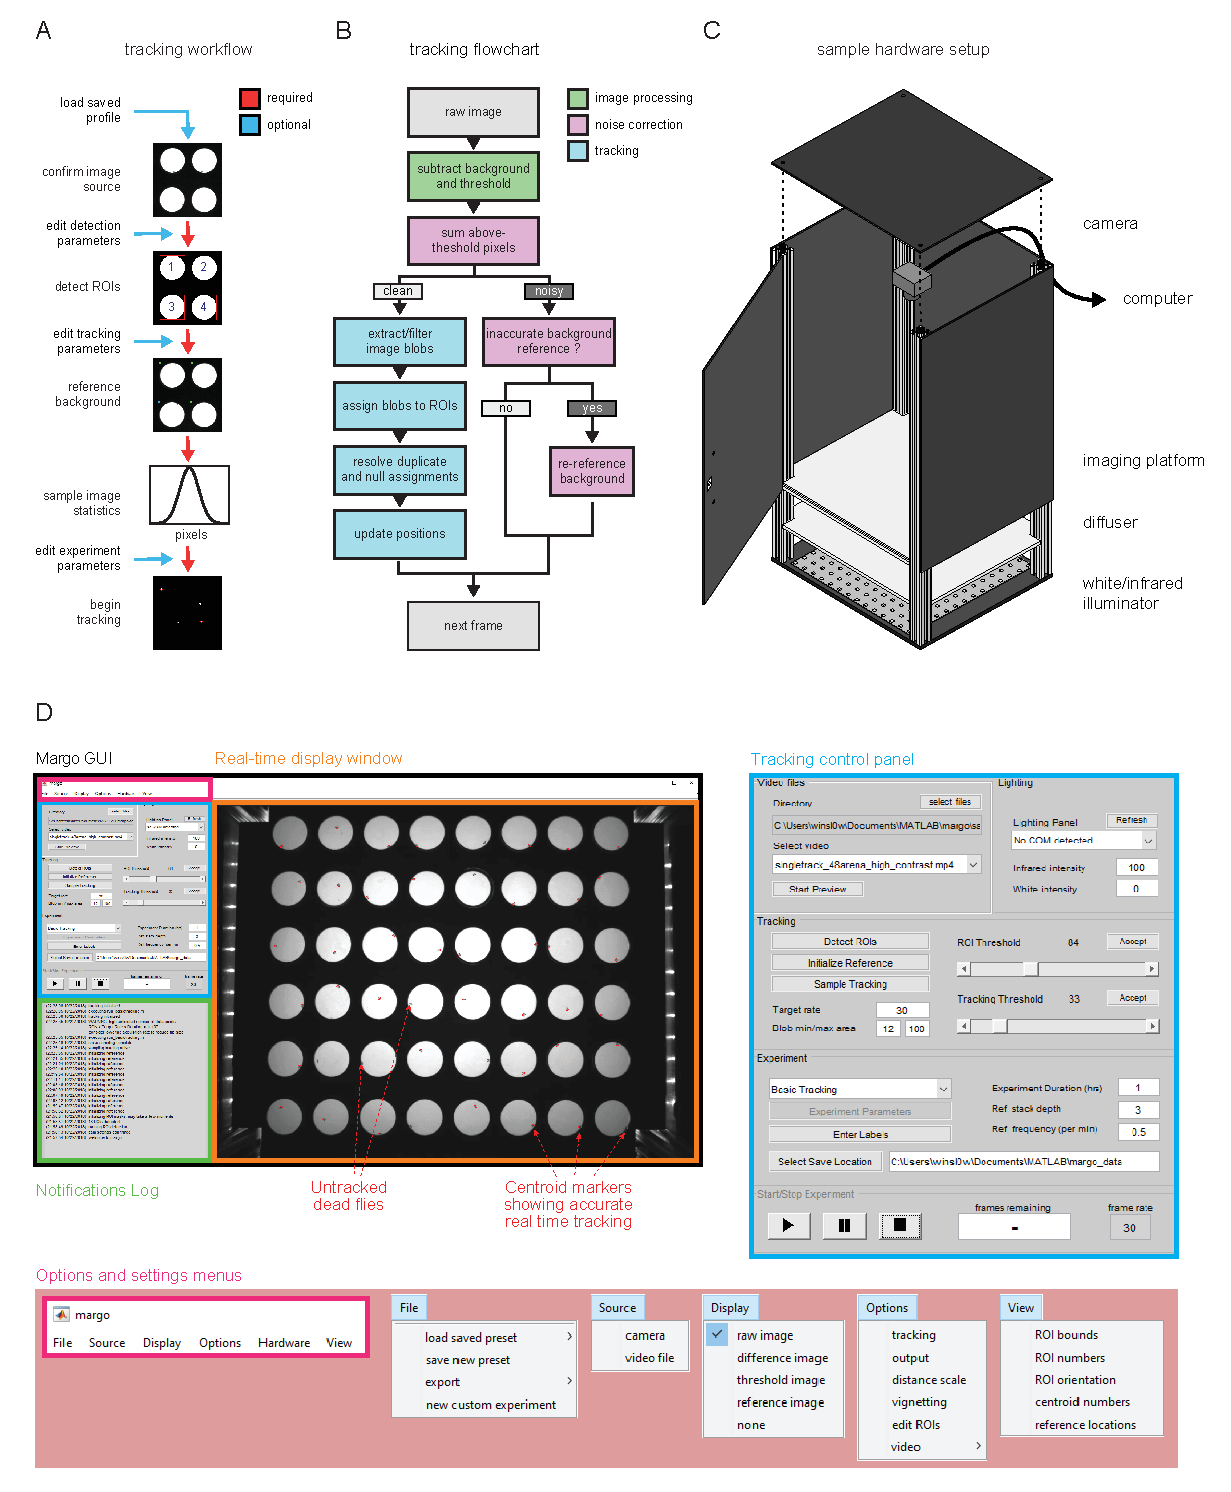
\includegraphics[width=0.9\textwidth]{../figures/autotracker_overview.pdf}
	\end{center}
	\caption*{\footnotesize \textbf{Figure 1. MARGO workflow, tracking algorithm, and sample behavioral box} -- A) Diagram of the user workflow to setup a new tracking experiment. Arrow color indicates whether the setup step is required. Before tracking, users define an input source, define ROIs to track, initialize a background reference used to separate foreground and background, and sample the image statistics on a reference of clean tracking. Multiple points are provided for customization of tracking parameters. B) Flowchart depicting the MARGO's frame-to-frame tracking routine. Each frame consists of image processing (green) to segment foreground from the background, noise estimation (magenta) to assess the quality of foreground segmentation and determine if the current frame can be tracked, and tracking (cyan) of foreground binary blobs. MARGO's tracking algorithm skips noisy frames and re-acquires the background reference if many consecutive frames are too noisy to track. C) Schematic of the behavioral boxes used to conduct tracking. Behavioral arenas are backlit with an LED illuminator and imaged with an overhead camera. The tracking camera is fitted with an infrared filter to allow light visible to the animals to be controled independently of the tracking illumination. A diffuser panel between the LED backlight and the behavioral arenas is used to achieve even illumination. The camera and LED backlight are both connected to computer for real-time tracking and control via MARGO.}
\end{figure}

\newpage
\begin{figure}[h!]
	\begin{center}
		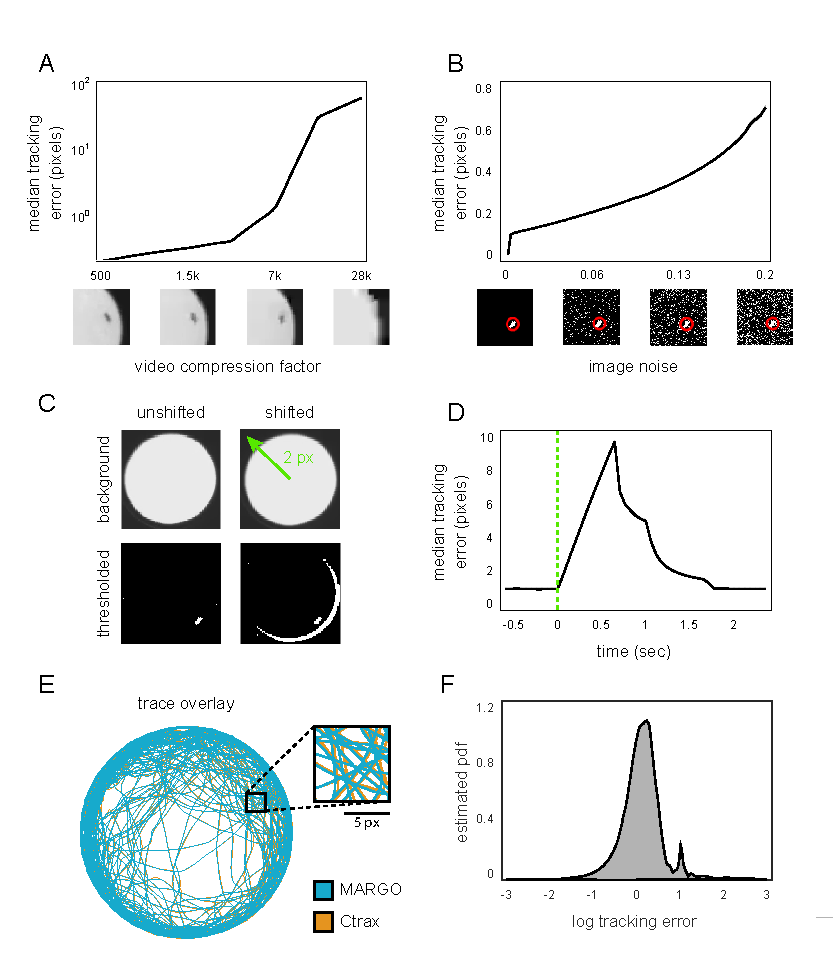
\includegraphics[width=0.9\textwidth]{../figures/autotracker_performance.pdf}
	\end{center}
	\caption*{\footnotesize \textbf{Figure 2. MARGO tracking accuracy is robust to video compression and imaging noise and is comparable Ctrax} -- A) Median [refraf replace with mean] error of tracking performed on the same video at different levels of compression. Sample images of the same fly and frame are shown below. B) Median [refraf replace with mean] error of tracking performed on the same video with different levels of added. Pixel noise was manually added to the binary threshold image downstream of image processing and noise detection by converting any given pixel to true at a fixed probability (image noise). Sample images of the same fly and frame, as well as estimated position (red circle) are shown below. C) Diagram of the background reference shifting scheme used to simulate background inaccuracy. D) Trial-triggered average tracking error centered on reference shifting. E-F) Sample trace comparison and log distribution of tracking error between traces acquired from the same video in both MARGO and Ctrax. The 95\% confidence interval of the above means were displayed but are within the thickness of lines.}
\end{figure}

\newpage
\begin{figure}[h!]
	\begin{center}
		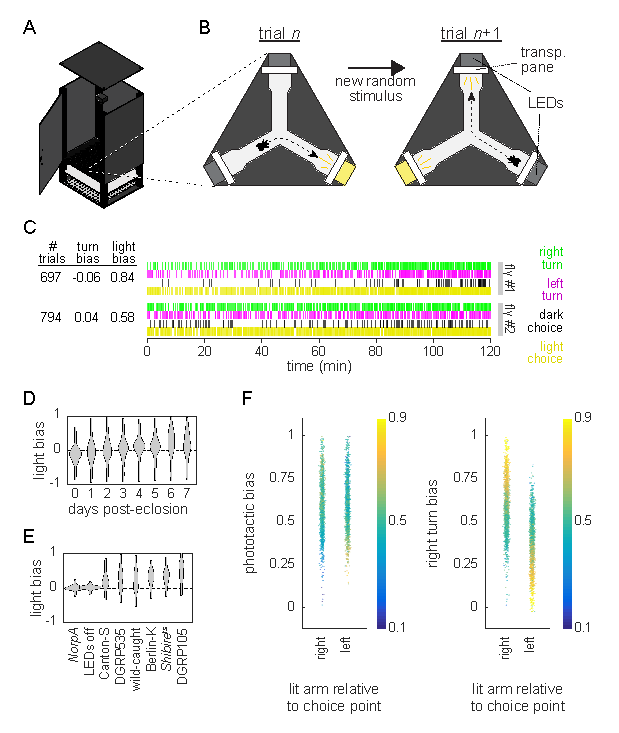
\includegraphics[width=0.9\textwidth]{../figures/LED_ymaze_panel.pdf}
	\end{center}
	\caption*{\footnotesize \textbf{Figure 3. High-throughput phototactic assay in Y-shaped arenas} -- A) Sample schematic of the LED Y-maze and behavioral box. B) Diagram of a single phototaxis maze and trial structure. New trials initiate by turning on (yellow) an LED in one of the two unoccupied maze arms. The trial ends when then animal turns into a new arm and the lit LED is turned off (gray). Each turn is scored for both handedness (left or right of the starting arm) and phototactic preference (positive or negative). C) Raw turn data for two sample flies. Individual means are typically averaged from hundreds of trials over a two hour period. D) Distribution of individual average phototactic biases for the same cohort of flies over the first 8 days post-eclosion. Horizontal dashed line indicates random bias at p=0.5. E) Comparison of individual average phototactic bias distributions for different wild-type flies. Blind flies (NorpA) and flies tested with all LEDs turned off (DGRP-105 dark) are included as negative controls.}
\end{figure}

\newpage
\begin{figure}[h!]
	\begin{center}
		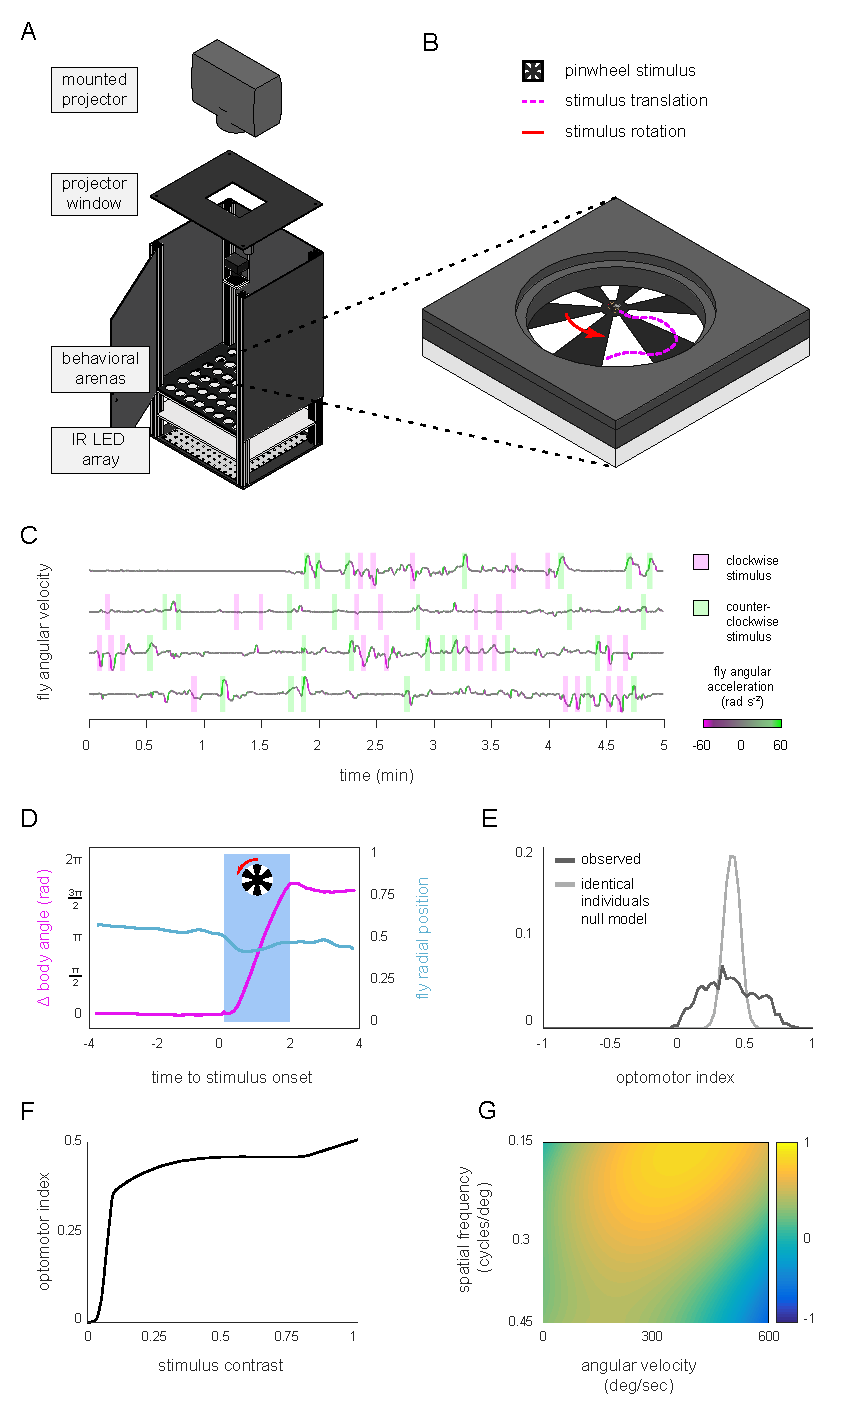
\includegraphics[width=0.5\textwidth]{../figures/Optomotor_panel.pdf}
	\end{center}
	\caption*{\footnotesize \textbf{Figure 4. High-throughput optomotor assay implementation in MARGO} -- A) Schematic of the optomotor arenas and behavioral box. B) Diagram of a single arena and optomotor stimulus. Trials begin with a displayed pinwheel stimulus centered on the body of the fly and rotating in a random direction (red arrow). The animal's tracked movement is used to maintain the stimulus center on estimated center of mass of the animal. Trials end when the stimulus is removed after a fixed duration (typically 2s). C) Sample raw individual time series data. Flies typically respond to optomotor stimuli by turning in the direction of the rotation of the stimulus. Hundreds of individual trials are recorded on average over a two hour period. D) Trial-triggered average optomotor response across all individuals. Positive change in body angle (magenta) is scored as rotation in the rotational direction of the stimulus. Average distance to the arena center (cyan) drops immediately preceeding stimulus onset due to the trial structure constraint that flies must be off the arena edge. E) Comparison of the observed distribution of individual average optomotor indeces (n=1,860) to an identical individuals null model. The null model distributions were generated by bootstrap resampling trials from the shared distribution of all trials up to a maximum number randomly sampled from observed individual trial numbers. F) Population average optomor index as a function of normalized stimulus contrast. Pinwheel contrast was randomly varied on a trial-by-trial basis. G) Population average optomor index as a function of stimulus spatial frequency and stimulus angular velocity. The 95\% confidence intervals of all above average traces are within the thickness of the line.}
\end{figure}

\newpage
\begin{figure}[t!]
	\begin{center}
		\vspace*{-8cm}
		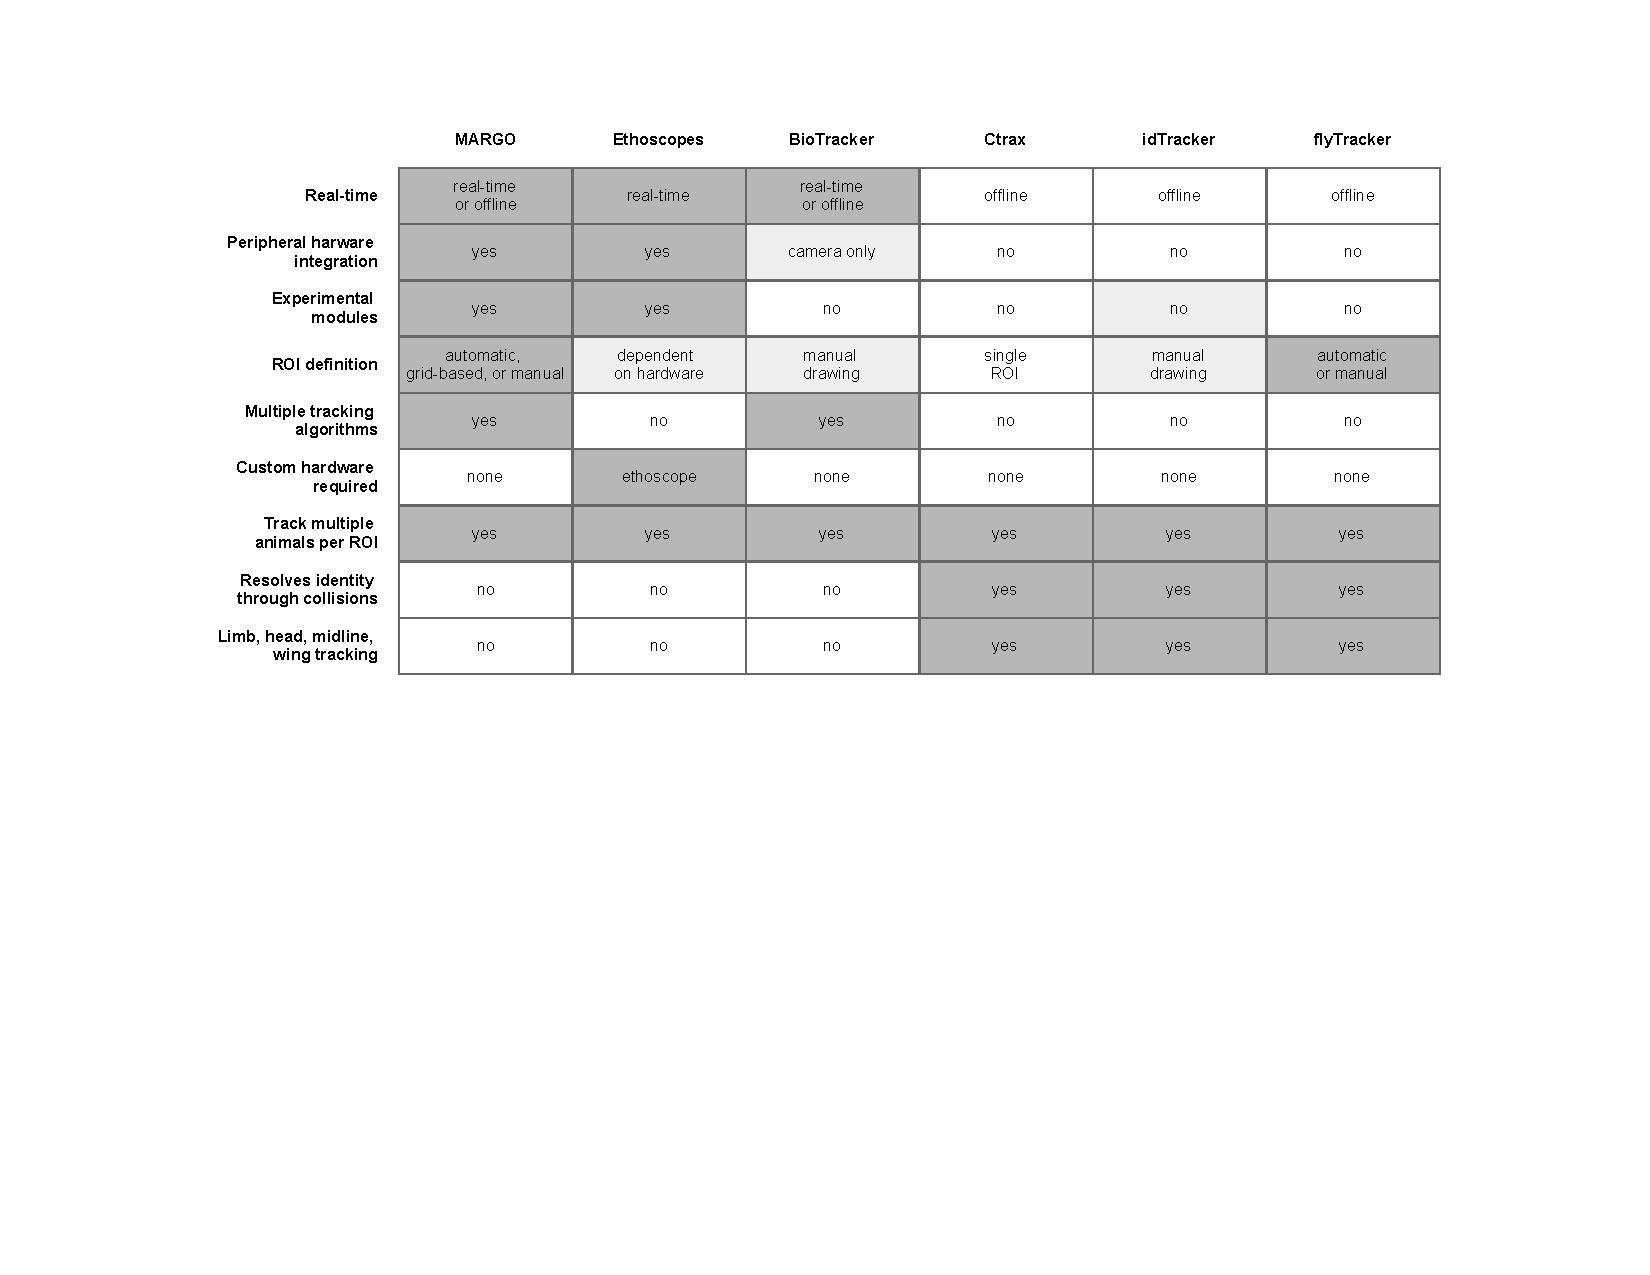
\includegraphics[width=0.9\textwidth]{../figures/platform_comparison_table.pdf}
	\end{center}
	\caption*{\footnotesize \textbf{Figure 5. Comparison of open-source animal tracking packages} -- Existing software packages offer a variety of features useful to ethologists. We see trackers as falling into one of two broad categories: 1) real-time trackers capable of very high-throughput with the potential hardware integration and stimulus delivery 2) off-line trackers capable of tracking postural features and maintaining individual identities without spatial segregation. We imagine MARGO, as well as other platforms such as Ethoscopes and BioTracker, falling into this first category. Experimental modules are a natural extension of real-time trackers since tracking and other specialized components of experiments needs can be conducted in parallel. Popular examples of programs in the second category include Ctrax, idTracker, and flyTracker. The comparably more computationally expensive tracking algorithms used as well as the training and calibration process make them unsuitable for real-time applications but offer the notable benefits of being able to study fine-scale postural and social behaviors.}
\end{figure}

\end{document}